% =====================================================================
%  FORM-IC-01 — Investigación individual: arquitecturas distribuidas
%  Caso: Nubank y su arquitectura orientada a eventos (EDA)
%  Aplicaciones Distribuidas — UTEQ — 7mo nivel, paralelo B
%
%  Compilación: pdflatex main.tex -> biber main -> pdflatex x2
% =====================================================================
\documentclass[11pt,a4paper]{article}

\usepackage[utf8]{inputenc}
\usepackage[T1]{fontenc}
\usepackage[english,spanish,es-tabla]{babel}
\usepackage[autostyle=true]{csquotes}
\usepackage{amsmath}

\usepackage[top=2.0cm,bottom=2.0cm,left=2.1cm,right=2.1cm]{geometry}
\usepackage{lmodern}
\usepackage{microtype}
\usepackage{parskip}
\usepackage{xcolor}

\usepackage{graphicx}
\usepackage{booktabs}
\usepackage{array}
\usepackage{caption}
\captionsetup{font=small,labelfont=bf,justification=justified}
\usepackage{float}

\usepackage{tikz}
\usetikzlibrary{calc}

\usepackage[style=ieee,backend=biber,sorting=none,language=english]{biblatex}
\addbibresource{../referencias.bib}

\usepackage[hidelinks]{hyperref}
\usepackage{url}

\usepackage{fancyhdr}
\setlength{\headheight}{15pt}
\pagestyle{fancy}
\fancyhf{}
\fancyhead[L]{\small Aplicaciones Distribuidas}
\fancyhead[R]{\small FORM-IC-01}
\fancyfoot[C]{\thepage}
\renewcommand{\headrulewidth}{0.4pt}

\usepackage{titlesec}
\titleformat{\section}{\normalfont\bfseries\large}{\thesection.}{0.5em}{}
\titlespacing*{\section}{0pt}{0.55ex plus 0.2ex minus 0.2ex}{0.25ex}

\setlength{\parindent}{0pt}
\setlength{\parskip}{0.25em}
\setlength{\abovedisplayskip}{2pt}
\setlength{\belowdisplayskip}{2pt}

\graphicspath{{../capturas/}{./}}

\begin{document}

% =====================================================================
%  CARÁTULA
% =====================================================================
\definecolor{verdeuteq}{HTML}{7CBA42}

\newcommand{\campoc}[2]{%
  \vspace{0.28cm}%
  {\bfseries #1\par}%
  \vspace{0.05cm}%
  {#2\par}}

\begin{titlepage}
\thispagestyle{empty}
\centering
\fontfamily{ptm}\selectfont

\begin{tikzpicture}[remember picture, overlay]
  \fill[verdeuteq] ([xshift=1.50cm,yshift=-1.11cm]current page.north west)
        rectangle ([xshift=19.48cm,yshift=-1.55cm]current page.north west);
  \fill[verdeuteq] ([xshift=1.50cm,yshift=-1.11cm]current page.north west)
        rectangle ([xshift=1.94cm,yshift=-28.20cm]current page.north west);
  \draw[black, line width=0.7pt]
        ([xshift=1.50cm,yshift=-1.11cm]current page.north west)
        rectangle ([xshift=19.58cm,yshift=-28.33cm]current page.north west);
\end{tikzpicture}

\vspace*{1.0cm}


\includegraphics[height=1.9cm]{logo-uteq.png}\hspace{1.9cm}%

\includegraphics[height=1.9cm]{logo-facultad.png}

\vspace{0.45cm}
{\Large\bfseries UNIVERSIDAD TÉCNICA ESTATAL DE QUEVEDO\par}
\vspace{0.24cm}
{\bfseries FACULTAD DE CIENCIAS DE LA COMPUTACIÓN Y DISEÑO DIGITAL\par}

\campoc{CARRERA:}{INGENIERÍA EN SOFTWARE 7MO NIVEL}
\campoc{ASIGNATURA:}{APLICACIONES DISTRIBUIDAS}
\campoc{DOCENTE:}{ING. GLEISTON CICERÓN GUERRERO ULLOA}
\campoc{TEMA:}{FORM-IC-01 — INVESTIGACIÓN INDIVIDUAL: ARQUITECTURAS\\DISTRIBUIDAS EN LA INDUSTRIA\\CASO: NUBANK Y SU ARQUITECTURA ORIENTADA A EVENTOS}
\campoc{ESTUDIANTE:}{MENDOZA BERMELLO ANGELLO AGUSTÍN}
\campoc{PARALELO:}{B}
\campoc{FECHA:}{26 DE NOVIEMBRE DE 2026}
\campoc{REPOSITORIO:}{\small\url{https://github.com/Amendozab5/FORM-IC-01-Nubank}}

\vspace{0.5cm}
{\bfseries AÑO LECTIVO 2026 — 2027\par}
\vspace{0.08cm}
{\itshape Quevedo — Los Ríos — Ecuador\par}

\end{titlepage}

% =====================================================================
%  ANÁLISIS DE UNA PÁGINA
% =====================================================================
\newpage
\begin{center}
{\Large\bfseries Nubank: 72\,000 millones de eventos diarios\\[0.1em]
en una arquitectura orientada a eventos\par}
\end{center}
\vspace{0.1cm}

\section{Descripción del caso}
Nubank es un banco digital brasileño con más de 110 millones de clientes en Brasil, Colombia y México. Su plataforma corre sobre más de 4\,000 microservicios en Kubernetes y procesa 72\,000 millones de eventos diarios a través de Kafka, con millones de peticiones por segundo \cite{nubank2025limits}. No es un experimento: es la infraestructura sobre la que se mueven cuentas, tarjetas, pagos y autorizaciones. La comunicación principal entre servicios es asíncrona; los servicios publican mensajes en un broker replicado y los consumen después \cite{nubank2019microservices}.

\section{Por qué eligió ese estilo y qué tenía antes}
Nubank nació en 2013 con un solo producto, tarjeta de crédito, y un solo país, Brasil. La arquitectura inicial era simple, como la de una startup \cite{nubank2025arch}. La empresa decidió empezar con microservicios desde el primer día, en contra del consejo de arrancar con un monolito. Rafael Ferreira, ingeniero de Nubank, reconoce el costo: montar la infraestructura de aprovisionamiento con un equipo pequeño los hizo más lentos al principio \cite{nubank2019microservices}. Aun así, prefirieron una base sólida antes que un modelo de cambios rápidos. La comunicación se resolvió con mensajería asíncrona: la mayor parte de las interacciones pasa por un broker replicado y, si un consumidor falla, el mensaje se desvía a una \emph{dead letter topic} en lugar de perderse \cite{nubank2019microservices}.

\section{Beneficios obtenidos}
El beneficio que más importa es organizacional. Con la estrategia multi-cuenta que llaman \emph{continental drift}, cada dominio puede tener su propia cuenta de AWS; un incidente en una cuenta no arrastra a las demás. Eso redujo el radio de fallo y aceleró los despliegues \cite{nubank2025limits}. La plataforma de tarjetas pasó de un servicio único a servicios flexibles que atienden la tarjeta combo en Brasil y las tarjetas separadas en México \cite{nubank2025arch}. La mensajería asíncrona permite que un equipo publique un evento y siga trabajando mientras otro lo consume a su ritmo.

\section{Desafíos y soluciones}
El primer desafío fue redibujar los límites: a medida que entendían el dominio, tenían que dividir o fusionar servicios, y eso sigue pasando \cite{nubank2019microservices}. El segundo fue el aprovisionamiento: pasaron por Chef, CoreOS Fleet, ECS, EC2 con CloudFormation y finalmente Kubernetes, con automatización para todos los recursos \cite{nubank2019microservices}. El tercero fue la consistencia: al ser asíncrono, el sistema no tiene una única verdad instantánea; Bação y Guerreiro separan la consistencia de datos, de proceso y de evolución \cite{bacao2026consistency}. Nubank la maneja con contratos estables para los datos analíticos y con \emph{dead letter topics} para no perder mensajes \cite{nubank2019microservices}. El cuarto fue la infraestructura: aunque la nube parezca infinita, las cuotas de AWS se convierten en un cuello de botella; construyeron un \emph{AWS Limit Smoke Detector} que compara uso, cuota y costo, y avisa antes del incidente \cite{nubank2025limits}. El quinto fue el radio de fallo, que atacaron con la estrategia multi-cuenta y el sharding de Datomic, Kafka y servicios \cite{nubank2025limits}. Söylemez agrupa esos problemas en nueve categorías \cite{soylemez2022challenges}, Bogner señala que el problema está en la arquitectura del conjunto \cite{bogner2021evolvability} y Abgaz confirma que la descomposición sigue sin estándares \cite{abgaz2023decomposition}.

\section{Aplicación al PFC}
El PFC del equipo es el Sistema de Pre-Sustentaciones: una aplicación web para solicitudes, documentos, revisiones, aprobaciones y notas, con un equipo pequeño y una base PostgreSQL. De Nubank tomaría los límites de dominio, los contratos estables y la idea de medir antes de separar. También tomaría la asincronía, pero solo para notificaciones, auditoría o tareas diferibles; no para el flujo de aprobación, donde el usuario necesita respuesta inmediata. No tomaría los 4\,000 servicios, el clúster de Kafka, la base por servicio ni las múltiples cuentas de AWS: son respuestas a una escala que el PFC no tiene. Blinowski muestra que en una sola máquina el monolito rinde mejor \cite{blinowski2022monolithic}; Al-Qora'n muestra que el monolito modular encaja cuando los microservicios cuestan más de lo que aportan \cite{alqoran2025modular}. Para el PFC, la opción sensata es un monolito modular con módulos claros, una sola base y medición de latencia y errores.

% =====================================================================
%  REFERENCIAS
% =====================================================================
\newpage
\selectlanguage{english}
\printbibliography[heading=bibintoc,title={Referencias}]
\selectlanguage{spanish}

% =====================================================================
%  ANEXO A — CAPTURA DE LA FUENTE PRINCIPAL
% =====================================================================
\newpage
\section*{Anexo A. Captura de la fuente principal}
\addcontentsline{toc}{section}{Anexo A. Captura de la fuente principal}

La captura corresponde a la entrada «Microservices at Nubank, an overview», de Rafael Ferreira, publicada el 12 de agosto de 2019 en el blog técnico oficial de Nubank. Los fragmentos amarillos marcan la decisión de empezar con microservicios desde 2013 y el reconocimiento de que esa decisión los hizo más lentos al inicio. El fragmento verde marca la consecuencia: los límites de los servicios se redibujan continuamente. Esa es la parte del caso que sostiene el análisis y la que se usa para explicar por qué el PFC no debe copiar la escala de Nubank.

\begin{center}
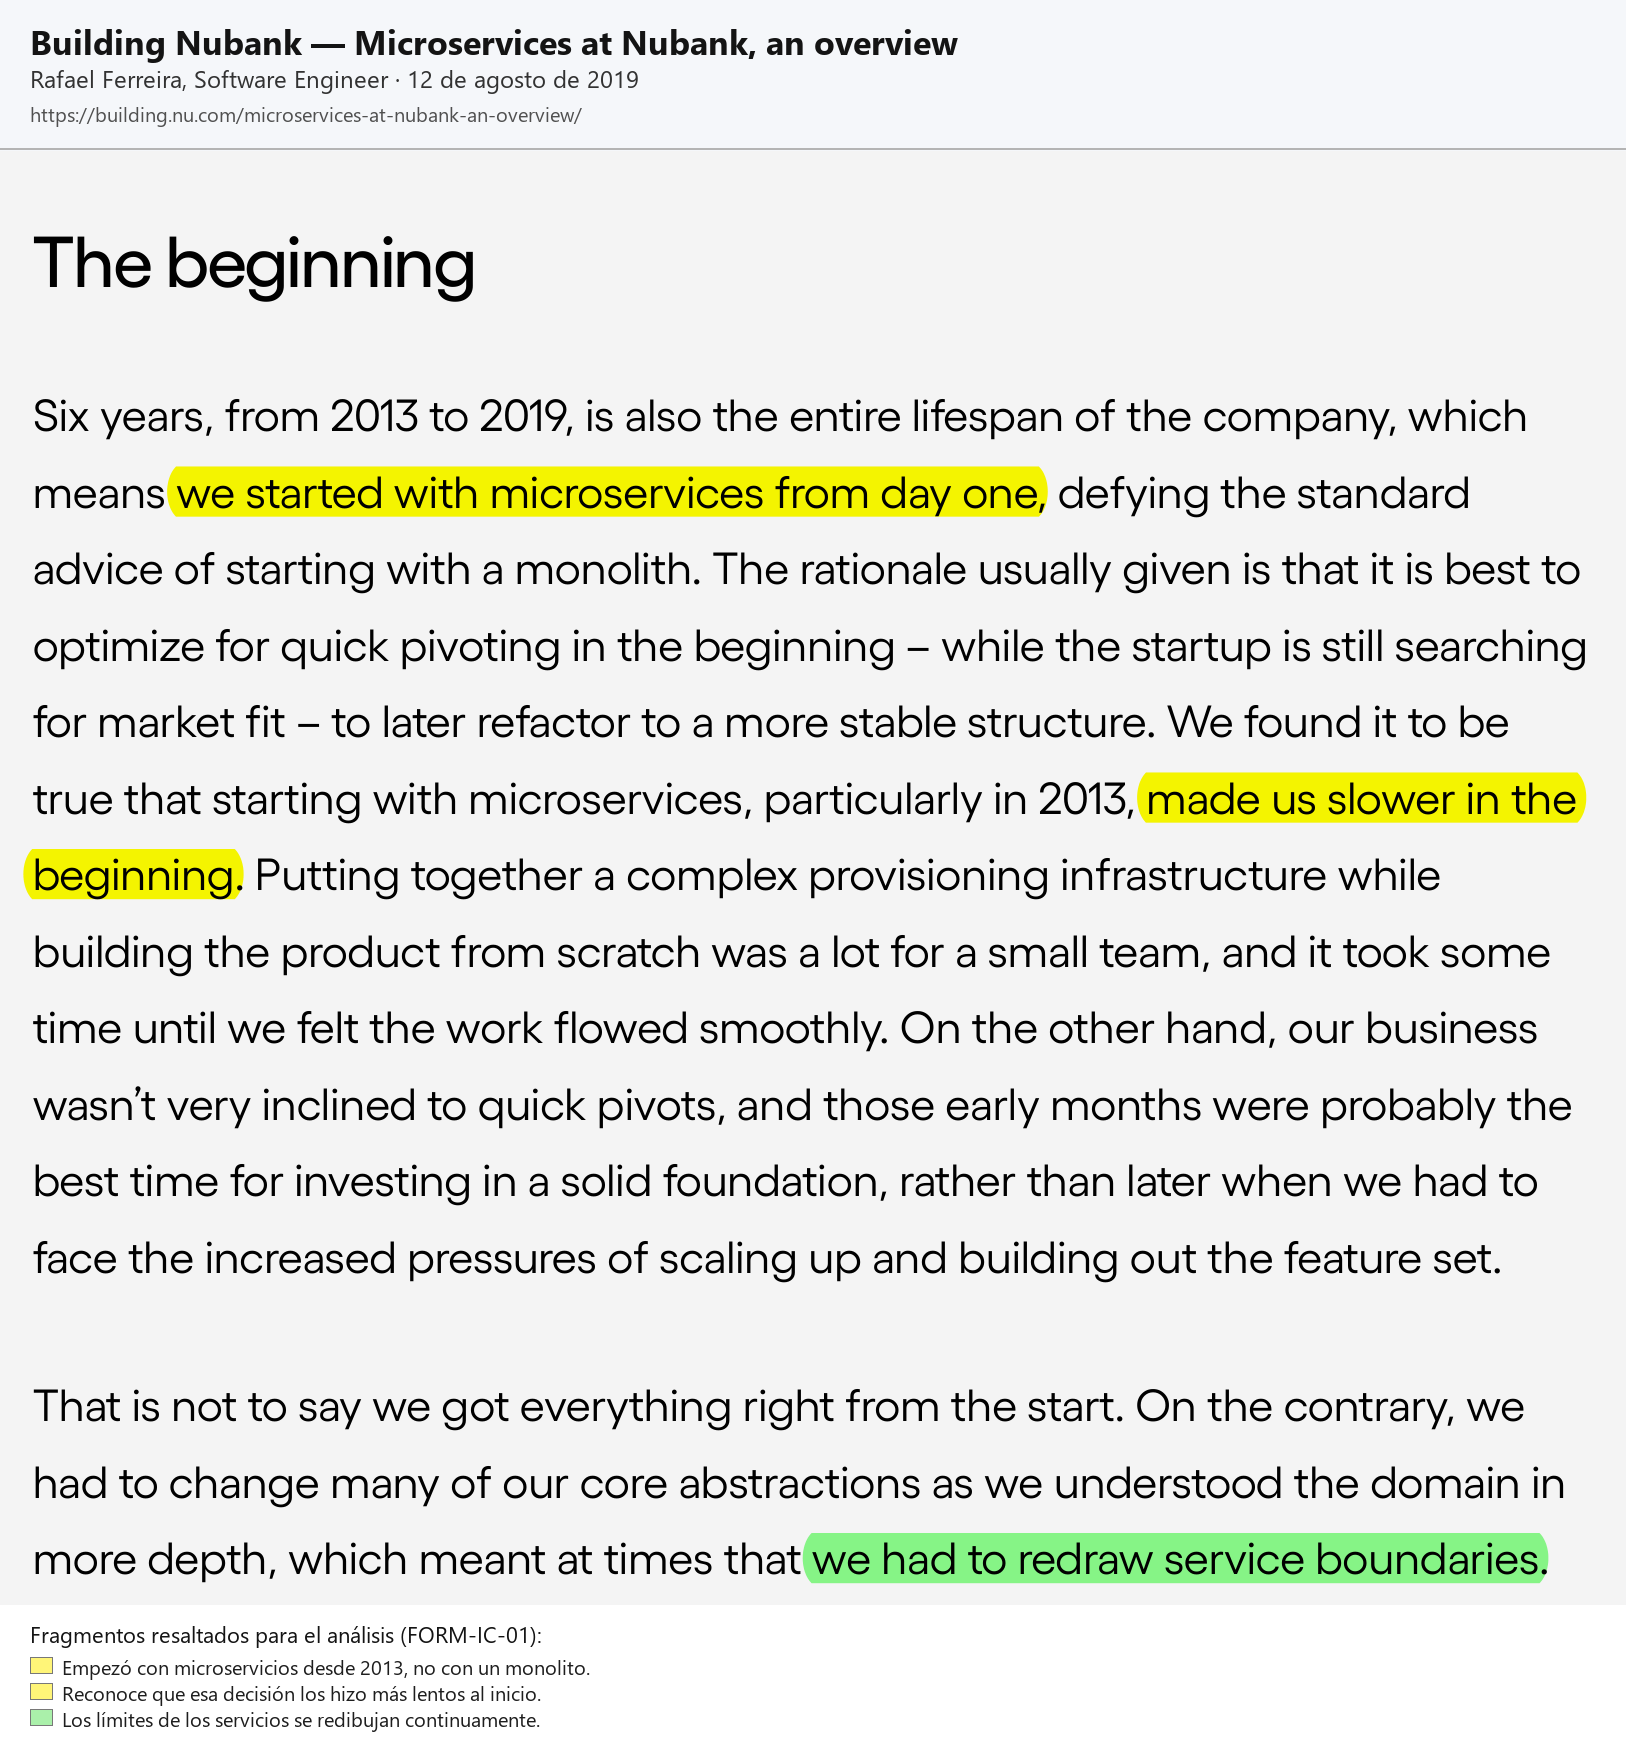
\includegraphics[width=0.95\textwidth,height=0.78\textheight,keepaspectratio]{01-fuente-nubank-anotada.png}
\end{center}

\clearpage
\section*{Anexo B. Sistema de primera mano}
\addcontentsline{toc}{section}{Anexo B. Sistema de primera mano}

El sistema de primera mano que uso todos los días es la aplicación móvil de mi banco. No veo su arquitectura por dentro, pero reconozco el patrón de Nubank en el comportamiento: la consulta de saldo, la transferencia y la notificación funcionan como piezas separadas. Cuando hago una transferencia, el débito se confirma antes de que llegue la notificación; si la sección de beneficios o promociones falla, la transferencia sigue funcionando. Esa separación entre la operación principal y los efectos secundarios es la misma idea que Nubank resuelve con un broker y mensajes asíncronos.

La diferencia es de evidencia. Nubank documenta el broker, las \emph{dead letter topics} y el sharding; en la aplicación del banco solo veo el resultado: la operación principal no espera a que termine la notificación. Esa observación me alcanza para reconocer el estilo, pero no para afirmar cómo está implementado. Por eso la tomo como un ejemplo de primera mano del patrón, no como una fuente técnica del caso.

\vspace{0.9cm}
\section*{Anexo C. Declaración de uso de inteligencia artificial}
\addcontentsline{toc}{section}{Anexo C. Declaración de uso de inteligencia artificial}

\textbf{Herramienta.} Asistente de programación DeepSeek Harness, modelo DeepSeek Flash, usado en sesión sobre el equipo local.

\textbf{Para qué.} Buscar candidatos de fuentes, ordenar el repositorio, revisar el formato LaTeX y proponer una estructura de redacción. También para generar la captura anotada a partir de la página oficial.

\textbf{Cómo se verificó.} Las cifras del caso salen del blog de Nubank y de los artículos descargados; no se tomaron de texto generado. Los datos bibliográficos se comprobaron uno por uno en Crossref y en la primera página de cada PDF. La captura se hizo sobre la página oficial de Nubank. La redacción final, la selección de las ideas y las decisiones de análisis son del estudiante.

\end{document}
